\documentclass[12pt,a4paper]{article}

% ─── Page Layout ───────────────────────────────────────────────────────────────
\usepackage[a4paper, margin=0.8in, headheight=14pt]{geometry}

% ─── Fonts (XeLaTeX) ───────────────────────────────────────────────────────────
\usepackage{fontspec}
\usepackage{unicode-math}
\setmainfont{TeX Gyre Pagella}
\setmonofont[Scale=0.88]{TeX Gyre Cursor}
\setmathfont{Latin Modern Math}

% ─── Packages ──────────────────────────────────────────────────────────────────
\usepackage{xcolor}
\usepackage{colortbl}
\usepackage{titlesec}
\usepackage{enumitem}
\usepackage{tabularx}
\usepackage{booktabs}
\usepackage{array}
\usepackage{amsmath}
\usepackage{tikz}
\usetikzlibrary{shapes.geometric, arrows.meta, positioning, calc, fit, decorations.pathreplacing}
\usepackage{tcolorbox}
\tcbuselibrary{skins, breakable}
\usepackage{hyperref}
\usepackage{fancyhdr}
\usepackage{graphicx}
\usepackage{microtype}
\hyphenpenalty=10000
\exhyphenpenalty=10000
\sloppy
\usepackage{caption}
\usepackage{setspace}
\usepackage{multirow}
\usepackage{tocloft}

% ─── Q&A helper ────────────────────────────────────────────────────────────────
\newcommand{\Q}[1]{\textbf{#1}\par\noindent\ignorespaces}

% ─── Colour Palette ────────────────────────────────────────────────────────────
\definecolor{myred}{RGB}{196,30,58}
\definecolor{mydark}{RGB}{30,30,50}
\definecolor{mygreen}{RGB}{14,120,80}
\definecolor{myteal}{RGB}{0,130,140}
\definecolor{myamber}{RGB}{180,100,0}
\definecolor{mypurple}{RGB}{100,30,160}
\definecolor{mygray}{RGB}{246,247,249}
\definecolor{mgframe}{RGB}{180,185,200}
\definecolor{watermark}{RGB}{145,150,170}
\definecolor{hdrred}{RGB}{250,232,235}
\definecolor{hdrgreen}{RGB}{220,244,233}
\definecolor{hdrteal}{RGB}{220,242,244}
\definecolor{hdramber}{RGB}{253,242,215}
\definecolor{hdrpurple}{RGB}{238,228,255}
\definecolor{hdrgray}{RGB}{238,240,245}
\definecolor{rowalt}{RGB}{250,251,253}

% ─── Section Formatting ────────────────────────────────────────────────────────
\titleformat{\section}
  {\large\bfseries\color{myred}}{\thesection.}{0.5em}{}
  [\vspace{1pt}{\color{myred}\rule{\linewidth}{0.8pt}}]
\titleformat{\subsection}
  {\normalsize\bfseries\color{myteal}}{\thesubsection}{0.5em}{}
\titlespacing*{\section}{0pt}{18pt}{7pt}
\titlespacing*{\subsection}{0pt}{11pt}{4pt}

% ─── Paragraph ─────────────────────────────────────────────────────────────────
\setlength{\parindent}{0pt}
\setlength{\parskip}{4pt}

% ─── TOC Styling ───────────────────────────────────────────────────────────────
\renewcommand{\cfttoctitlefont}{\large\bfseries\color{myred}}
\renewcommand{\cftaftertoctitle}{\par\noindent{\color{myred}\rule{\linewidth}{0.8pt}}}
\setlength{\cftbeforetoctitleskip}{0pt}
\setlength{\cftaftertoctitleskip}{6pt}
\renewcommand{\cftsecfont}{\normalsize\bfseries\color{mydark}}
\renewcommand{\cftsecpagefont}{\normalsize\bfseries\color{mydark}}
\renewcommand{\cftsecleader}{\cftdotfill{\cftdotsep}}
\setlength{\cftbeforesecskip}{7pt}
\renewcommand{\cftsubsecfont}{\small\color{mydark}}
\renewcommand{\cftsubsecpagefont}{\small\color{mydark}}
\setlength{\cftbeforesubsecskip}{3pt}
\setlength{\cftsubsecindent}{1.4em}

% ─── Table helpers ─────────────────────────────────────────────────────────────
\renewcommand{\arraystretch}{1.45}
\setlength{\tabcolsep}{6pt}
\arrayrulecolor{mydark}
\newcolumntype{B}[1]{>{\small\bfseries\raggedright\arraybackslash}m{#1}}
\newcolumntype{Y}{>{\small\raggedright\arraybackslash}X}
\renewcommand{\tabularxcolumn}[1]{m{#1}}

% ─── Header / Footer ───────────────────────────────────────────────────────────
\pagestyle{fancy}
\fancyhf{}
\fancyhead[L]{\small\color{myred}\textbf{PE-EC701C}\;\color{mydark}--- Mobile Communication and Networks}
\fancyhead[R]{\small\color{myteal}\textbf{Module 4 Notes}}
\fancyfoot[C]{\small\color{mydark}\thepage}
\fancyfoot[R]{\small\color{watermark}\textit{\copyright\ Biraj}}
\renewcommand{\headrulewidth}{0.5pt}
\renewcommand{\footrulewidth}{0.3pt}

% ─── Hyperref ──────────────────────────────────────────────────────────────────
\hypersetup{
  colorlinks=true, linkcolor=myteal, urlcolor=myteal,
  pdfauthor={Biraj Sarkar},
  pdftitle={PE-EC701C --- Module 4 Notes}
}

% ─── tcolorbox styles ──────────────────────────────────────────────────────────
\tcbset{
  tikzbox/.style={
    colback=mygray, colframe=mgframe, boxrule=0.6pt, arc=4pt,
    left=8pt, right=8pt, top=6pt, bottom=6pt,
    colbacktitle=mgframe, coltitle=mydark,
    fonttitle=\small\bfseries
  },
  defbox/.style={
    colback=hdrgreen, colframe=mygreen, boxrule=0.8pt, arc=4pt,
    left=9pt, right=9pt, top=6pt, bottom=6pt,
    colbacktitle=mygreen, coltitle=white,
    fonttitle=\small\bfseries
  },
  formulabox/.style={
    colback=hdrteal, colframe=myteal, boxrule=0.8pt, arc=4pt,
    left=9pt, right=9pt, top=7pt, bottom=7pt,
    colbacktitle=myteal, coltitle=white,
    fonttitle=\small\bfseries
  },
  examplebox/.style={
    colback=hdramber, colframe=myamber, boxrule=0.8pt, arc=4pt,
    left=9pt, right=9pt, top=6pt, bottom=6pt,
    colbacktitle=myamber, coltitle=white,
    fonttitle=\small\bfseries
  },
  masonbox/.style={
    colback=hdrpurple, colframe=mypurple, boxrule=0.8pt, arc=4pt,
    left=9pt, right=9pt, top=6pt, bottom=6pt,
    colbacktitle=mypurple, coltitle=white,
    fonttitle=\small\bfseries
  },
  exambox/.style={
    colback=hdrpurple, colframe=mypurple, boxrule=1pt, arc=5pt,
    left=10pt, right=10pt, top=8pt, bottom=8pt,
    colbacktitle=mypurple, coltitle=white,
    fonttitle=\bfseries,
    breakable, title after break={\textbf{Frequently Asked / Viva Questions (contd.)}}}
}
\tcbset{breakable}

% ─── TikZ styles ───────────────────────────────────────────────────────────────
\tikzset{
  block/.style={rectangle, draw=myteal, fill=hdrteal,
    text width=2.4cm, align=center, minimum height=0.95cm,
    font=\small, rounded corners=3pt, line width=0.7pt},
  redblock/.style={rectangle, draw=myred, fill=hdrred,
    text width=2.4cm, align=center, minimum height=0.95cm,
    font=\small, rounded corners=3pt, line width=0.7pt},
  netnode/.style={rectangle, draw=myteal, fill=hdrteal,
    text width=1.5cm, align=center, minimum height=0.8cm,
    font=\small, rounded corners=3pt, line width=0.7pt},
  sumjunc/.style={circle, draw=myamber, fill=hdramber,
    minimum size=0.62cm, font=\small, line width=0.8pt},
  snode/.style={circle, draw=mypurple, fill=hdrpurple,
    minimum size=0.55cm, font=\footnotesize, line width=0.7pt},
  arrow/.style={-Stealth, thick, color=mydark},
  redarrow/.style={-Stealth, thick, color=myred},
  line/.style={thick, color=mydark}
}

% ═══════════════════════════════════════════════════════════════════════════════
\begin{document}
% ═══════════════════════════════════════════════════════════════════════════════

\begin{center}
  {\LARGE\bfseries\color{myred} PE-EC701C --- Mobile Communication and Networks}\\[5pt]
  {\normalsize\color{mydark} Semester VII \quad$\bullet$\quad 3L:0T:0P \quad$\bullet$\quad 3 Credits}\\[3pt]
  {\normalsize\color{myteal}\textbf{Module 4 Exam Notes: Multiple Access and Modulation Schemes}}\\[3pt]
  {\small\color{mydark} CGEC \;$|$\; B.Tech ECE (2023--27) \;$|$\; \textit{Biraj Sarkar}}
\end{center}
\noindent{\color{myred}\rule{\linewidth}{1.5pt}}
\vspace{2pt}

\hypersetup{linkcolor=mydark}
\tableofcontents
\hypersetup{linkcolor=myteal}
\newpage

% ===============================================================================
\section{Multiple Access Schemes}
% ===============================================================================

Multiple access schemes allow many mobile users to share the same physical radio spectrum simultaneously without causing mutual interference.

\subsection{FDMA, TDMA, CDMA, and SDMA}
\begin{itemize}[leftmargin=*, itemsep=3.5pt]
  \item \textbf{FDMA (Frequency Division Multiple Access):} Divides the allocated spectrum into narrow, non-overlapping frequency channels. Each user is assigned a unique channel for the duration of the call. Requires guard bands to prevent adjacent channel interference. Used in 1G systems.
  \item \textbf{TDMA (Time Division Multiple Access):} Divides a single carrier frequency channel into multiple non-overlapping time slots. Each user is assigned a specific slot periodically, transmitting in bursts. Requires guard times to prevent slot overlaps. Used in GSM (2G).
  \item \textbf{CDMA (Code Division Multiple Access):} Users share the entire allocated bandwidth simultaneously. Each user's signal is multiplied by a unique, orthogonal pseudo-noise (PN) code. The receiver uses the same code to despread and recover the desired signal while treating other users' signals as wideband noise. Used in IS-95 (2G) and WCDMA (3G).
  \item \textbf{SDMA (Spatial Division Multiple Access):} Serves different users on the same frequency and time by using highly directional smart antennas (beamforming) to separate signals spatially.
\end{itemize}

\begin{tcolorbox}[tikzbox, title={TDMA Frame and Slot Structure}]
\centering
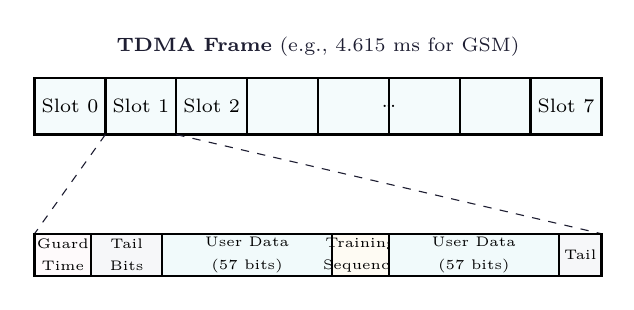
\begin{tikzpicture}[scale=0.9, every node/.style={font=\scriptsize}]
  % Draw TDMA Frame
  \draw[thick, fill=hdrteal!30] (0,1.2) rectangle (8,2.0);

  % Split slots
  \foreach \x in {1,2,3,4,5,6,7} {
    \draw[thick] (\x,1.2) -- (\x,2.0);
  }
  \node at (0.5, 1.6) {Slot 0};
  \node at (1.5, 1.6) {Slot 1};
  \node at (2.5, 1.6) {Slot 2};
  \node at (7.5, 1.6) {Slot 7};
  \node at (5.0, 1.6) {\dots};

  % Frame Label above
  \node[above=0.15cm, color=mydark] at (4, 2.0) {\textbf{TDMA Frame} (e.g., 4.615 ms for GSM)};

  % Expand Slot 1
  \draw[dashed, color=mydark] (1.0, 1.2) -- (0, -0.2);
  \draw[dashed, color=mydark] (2.0, 1.2) -- (8.0, -0.2);

  % Detail Slot structure
  \draw[thick, fill=hdrred!20] (0,-0.2) rectangle (0.8,-0.8) node[midway, align=center] {\tiny Guard\\ \tiny Time};
  \draw[thick, fill=mygray] (0.8,-0.2) rectangle (1.8,-0.8) node[midway, align=center] {\tiny Tail\\ \tiny Bits};
  \draw[thick, fill=hdrteal!40] (1.8,-0.2) rectangle (4.2,-0.8) node[midway, align=center] {\tiny User Data\\ \tiny (57 bits)};
  \draw[thick, fill=hdramber!30] (4.2,-0.2) rectangle (5.0,-0.8) node[midway, align=center] {\tiny Training\\ \tiny Sequence};
  \draw[thick, fill=hdrteal!40] (5.0,-0.2) rectangle (7.4,-0.8) node[midway, align=center] {\tiny User Data\\ \tiny (57 bits)};
  \draw[thick, fill=mygray] (7.4,-0.2) rectangle (8.0,-0.8) node[midway, align=center] {\tiny Tail};
\end{tikzpicture}
\end{tcolorbox}

% ===============================================================================
\section{Modulation Schemes in Mobile Communications}
% ===============================================================================

Mobile radio channels require modulation schemes that are spectrally efficient, robust against multipath distortion, and power efficient (low peak-to-average power ratio).

\subsection{BPSK, QPSK, and Variants}
\begin{itemize}[leftmargin=*, itemsep=3.0pt]
  \item \textbf{BPSK (Binary Phase Shift Keying):} Maps 1 bit per symbol to phases $0$ and $\pi$. Simple and robust, but has low spectral efficiency ($1\,\text{bps/Hz}$).
  \item \textbf{QPSK (Quadrature Phase Shift Keying):} Maps 2 bits per symbol to four phases ($45^\circ$, $135^\circ$, $225^\circ$, $315^\circ$). Achieves double the spectral efficiency of BPSK ($2\,\text{bps/Hz}$) within the same bandwidth.
  \item \textbf{OQPSK (Offset QPSK):} Introduces a $T_s/2$ time delay between the in-phase ($I$) and quadrature ($Q$) bit streams. This prevents simultaneous transitions of both streams, limiting phase changes to a maximum of $90^\circ$ (instead of $180^\circ$ in standard QPSK). This reduces envelope fluctuations after filtering, allowing efficient non-linear amplifiers.
  \item \textbf{$\pi/4$-DQPSK (Differential QPSK):} The phase constellation rotates by $\pi/4$ every symbol interval. The maximum phase change is limited to $135^\circ$, which prevents the signal envelope from passing through zero. This reduces spectral regrowth and simplifies demodulation using differential detection.
\end{itemize}

\subsection{MSK and GMSK}
Non-constant envelope signals experience severe distortion when passed through non-linear power amplifiers. Constant envelope modulation schemes solve this issue:
\begin{itemize}[leftmargin=*, itemsep=3pt]
  \item \textbf{MSK (Minimum Shift Keying):} A continuous-phase frequency shift keying (CPFSK) scheme with a modulation index $m = 0.5$ (minimum frequency spacing for orthogonal detection). The phase changes linearly over each symbol period.
  \item \textbf{GMSK (Gaussian Minimum Shift Keying):} Derived from MSK by filtering the baseband NRZ data stream through a Gaussian low-pass filter before frequency modulation.
    \begin{itemize}[leftmargin=*, itemsep=2pt, topsep=2pt]
      \item \textbf{Advantage:} The Gaussian filter smooths the phase transitions, suppressing the side lobes of the transmitted spectrum. This minimizes adjacent channel interference (ACI).
      \item \textbf{Trade-off:} The smoothing introduces controlled Inter-Symbol Interference (ISI) in the time domain, requiring an equalizer at the receiver. Used in the GSM standard.
    \end{itemize}
\end{itemize}

\begin{tcolorbox}[tikzbox, title={GMSK Transmitter Block Diagram}]
\centering
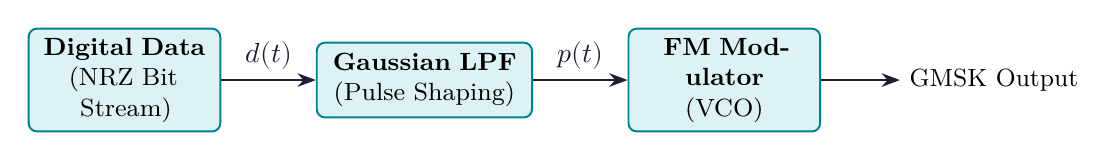
\begin{tikzpicture}[node distance=0.6cm and 1.2cm]
  \node[block, text width=2.2cm] (data) {\textbf{Digital Data}\\(NRZ Bit Stream)};
  \node[block, right=1.2cm of data, text width=2.5cm] (gauss) {\textbf{Gaussian LPF}\\(Pulse Shaping)};
  \node[block, right=1.2cm of gauss, text width=2.2cm] (mod) {\textbf{FM Modulator}\\(VCO)};
  \node[right=1.0cm of mod] (out) {\small GMSK Output};
  
  \draw[arrow] (data) -- (gauss) node[midway, above] {$d(t)$};
  \draw[arrow] (gauss) -- (mod) node[midway, above] {$p(t)$};
  \draw[arrow] (mod) -- (out);
\end{tikzpicture}
\end{tcolorbox}

% ===============================================================================
\section{Multicarrier Modulation and OFDM}
% ===============================================================================

\subsection{Basic Principles of OFDM}
Orthogonal Frequency Division Multiplexing (OFDM) is a multicarrier modulation scheme that divides a high-speed data stream into multiple parallel, low-speed streams modulated onto orthogonal subcarriers.

\begin{tcolorbox}[defbox]
\textbf{Subcarrier Orthogonality:} Two subcarriers are orthogonal if their frequencies are spaced at multiples of the inverse of the symbol duration ($1/T$). Mathematically:
\begin{equation}
  \frac{1}{T}\int_{0}^{T} e^{j 2\pi f_m t} \cdot e^{-j 2\pi f_n t} \, dt = 0 \quad (\text{for } f_m - f_n = \frac{k}{T}, \; k \neq 0)
\end{equation}
This allows their spectra to overlap in the frequency domain without causing mutual interference (ICI), maximizing spectral efficiency.
\end{tcolorbox}

\subsection{Mathematical Formulation (IFFT/FFT Relation)}
An OFDM symbol is generated in the digital domain using the Inverse Fast Fourier Transform (IFFT). Let $X_k$ be the complex modulation symbol (e.g., QAM) mapped to the $k$-th subcarrier. The discrete-time baseband OFDM signal is:
\begin{equation}
  x(n) = \frac{1}{\sqrt{N}} \sum_{k=0}^{N-1} X_k e^{j \frac{2\pi k n}{N}} \quad \implies \text{IDFT / IFFT operation}
\end{equation}
At the receiver, the symbols are recovered using the Fast Fourier Transform (FFT):
\begin{equation}
  X_k = \frac{1}{\sqrt{N}} \sum_{n=0}^{N-1} x(n) e^{-j \frac{2\pi k n}{N}} \quad \implies \text{DFT / FFT operation}
\end{equation}

\subsection{Cyclic Prefix (CP) Insertion}
To eliminate Inter-Symbol Interference (ISI) caused by multipath delay spread, a \textbf{Cyclic Prefix (CP)} is appended to the beginning of each OFDM symbol.
\begin{itemize}[leftmargin=*, itemsep=3.0pt]
  \item \textbf{Mechanism:} The CP is a copy of the end portion of the OFDM symbol, prepended to the start. The duration of the CP ($T_{\text{CP}}$) must be longer than the maximum delay spread of the channel ($\tau_{\text{max}}$).
  \item \textbf{Purpose:} 
    \begin{itemize}[leftmargin=*, itemsep=2pt, topsep=2pt]
      \item Acts as a guard time, preventing the preceding symbol's multipath components from interfering with the current symbol (eliminates ISI).
      \item Converts linear channel convolution into circular convolution, allowing simple one-tap frequency-domain equalization (FDE) at the receiver.
    \end{itemize}
\end{itemize}

\subsection{Peak-to-Average Power Ratio (PAPR) Issue}
The primary drawback of OFDM is its high PAPR.
\begin{itemize}[leftmargin=*, itemsep=3.5pt]
  \item \textbf{Cause:} Because an OFDM symbol is the sum of many independent subcarriers, their constructive phase alignment can produce large peak signals relative to the average power.
  \item \textbf{Impact:} High PAPR requires power amplifiers with wide linear ranges, reducing efficiency and increasing costs. Non-linear amplification causes out-of-band emissions and in-band distortion.
  \item \textbf{Mitigation:} Clipping and filtering, selective mapping (SLM), coding (e.g., Golay complementary sequences), and using Single-Carrier FDMA (SC-FDMA) on the uplink (as in LTE).
\end{itemize}

\begin{tcolorbox}[tikzbox, title={OFDM Transmitter and Receiver Block Diagrams}]
\centering
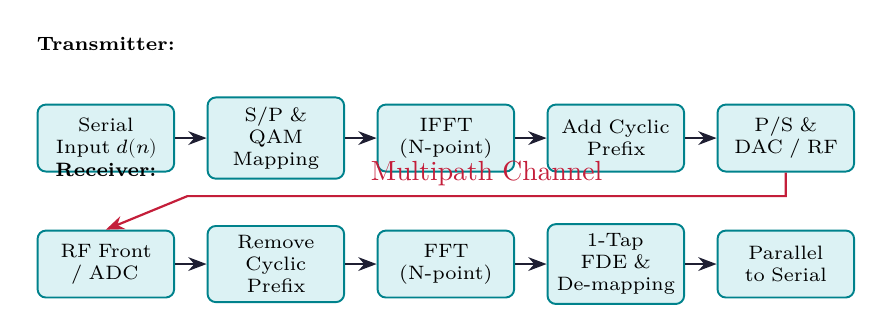
\begin{tikzpicture}[node distance=0.35cm and 0.55cm,
  sblock/.style={rectangle, draw=myteal, fill=hdrteal, text width=1.5cm,
    align=center, minimum height=0.85cm, font=\scriptsize,
    rounded corners=3pt, line width=0.7pt}]

  % Transmitter
  \node[font=\scriptsize\bfseries] at (0,1.2) {Transmitter:};
  \node[sblock] (tx_in) {Serial Input $d(n)$};
  \node[sblock, right=0.4cm of tx_in] (tx_s2p) {S/P \& QAM Mapping};
  \node[sblock, right=0.4cm of tx_s2p] (tx_ifft) {IFFT\\(N-point)};
  \node[sblock, right=0.4cm of tx_ifft] (tx_cp) {Add Cyclic Prefix};
  \node[sblock, right=0.4cm of tx_cp] (tx_p2s) {P/S \& DAC / RF};
  \draw[arrow] (tx_in) -- (tx_s2p);
  \draw[arrow] (tx_s2p) -- (tx_ifft);
  \draw[arrow] (tx_ifft) -- (tx_cp);
  \draw[arrow] (tx_cp) -- (tx_p2s);

  % Receiver
  \node[font=\scriptsize\bfseries] at (0,-0.4) {Receiver:};
  \begin{scope}[shift={(0,-1.6)}]
    \node[sblock] (rx_in) {RF Front / ADC};
    \node[sblock, right=0.4cm of rx_in] (rx_cp) {Remove Cyclic Prefix};
    \node[sblock, right=0.4cm of rx_cp] (rx_fft) {FFT\\(N-point)};
    \node[sblock, right=0.4cm of rx_fft] (rx_eq) {1-Tap FDE \& De-mapping};
    \node[sblock, right=0.4cm of rx_eq] (rx_out) {Parallel to Serial};
    \draw[arrow] (rx_in) -- (rx_cp);
    \draw[arrow] (rx_cp) -- (rx_fft);
    \draw[arrow] (rx_fft) -- (rx_eq);
    \draw[arrow] (rx_eq) -- (rx_out);
  \end{scope}

  % Connect Tx to Rx
  \draw[arrow, redarrow] (tx_p2s.south) -- +(0,-0.3) -- node[midway, above, color=myred] {Multipath Channel} +(-7.6,-0.3) -- (rx_in.north);
\end{tikzpicture}
\end{tcolorbox}

% ===============================================================================
% MANDATORY QUICK REVISION PAGE
% ===============================================================================
\newpage
\begin{center}
  {\large\bfseries\color{myred} Quick Revision --- Module IV}\\[3pt]
  {\small\color{mydark} Multiple Access and Modulation Schemes $|$ PE-EC701C}
\end{center}
\noindent{\color{myred}\rule{\linewidth}{1.2pt}}
\vspace{4pt}

\begin{tcolorbox}[formulabox, title={\textbf{Key Formulas at a Glance}}]
\renewcommand{\arraystretch}{1.3}
\begin{tabularx}{\linewidth}{B{5.5cm} X}
Subcarrier Frequency Spacing & $\Delta f = \frac{1}{T}$ \quad ($T$ = active OFDM symbol duration) \\
OFDM Subcarrier Orthogonality & $\frac{1}{T}\int_{0}^{T} e^{j 2\pi f_m t} \cdot e^{-j 2\pi f_n t} \, dt = 0 \quad (f_m - f_n = \frac{k}{T})$ \\
Discrete OFDM Signal (IFFT) & $x(n) = \frac{1}{\sqrt{N}} \sum_{k=0}^{N-1} X_k e^{j \frac{2\pi k n}{N}}$ \\
Cyclic Prefix Condition & $T_{\text{CP}} \ge \tau_{\text{max}}$ \quad ($\tau_{\text{max}}$ = max channel delay spread) \\
Peak-to-Average Power Ratio & $\text{PAPR} = \frac{\max |x(t)|^2}{\mathbb{E}[|x(t)|^2]}$ \\
MSK Frequency Separation & $\Delta f_{\text{min}} = \frac{1}{2T_b}$ \quad (minimum for coherent orthogonality)
\end{tabularx}
\end{tcolorbox}

\begin{tcolorbox}[defbox, title={\textbf{One-Line Definitions}}]
\begin{itemize}[leftmargin=*, itemsep=2.5pt, topsep=0pt]
  \item \textbf{FDMA:} Allocates unique, narrow frequency bands to users for the duration of the call.
  \item \textbf{TDMA:} Divides the carrier frequency into periodic time slots, assigning one to each user.
  \item \textbf{CDMA:} Allows users to share the entire bandwidth simultaneously using unique orthogonal codes.
  \item \textbf{Offset QPSK:} A QPSK variant that delays the Q-channel by half a symbol period to prevent envelope drops.
  \item \textbf{GMSK:} A continuous-phase modulation scheme that shapes baseband pulses using a Gaussian filter before modulation.
  \item \textbf{OFDM:} A multicarrier modulation scheme dividing a high-rate stream into orthogonal, overlapping subchannels.
  \item \textbf{Cyclic Prefix:} A copy of the end of an OFDM symbol prepended to the start to eliminate ISI.
\end{itemize}
\end{tcolorbox}

\begin{tcolorbox}[exambox, title={\textbf{Frequently Asked / Viva Questions}}]
\begin{enumerate}[topsep=0pt, label=\textbf{Q\arabic*.}, itemsep=5pt]
  \item \Q{What is the primary difference between TDMA and FDMA regarding slot guard times?}
    TDMA requires guard times between time slots to prevent overlapping from propagation delays. FDMA requires guard bands in the frequency domain to prevent adjacent channel interference.
  \item \Q{Explain the physical meaning of orthogonality in OFDM.}
    Subcarrier frequencies are spaced at multiples of the inverse of the symbol duration ($1/T$). At the peak of any single subcarrier's spectrum, the spectra of all other subcarriers are zero, preventing inter-carrier interference.
  \item \Q{Why does GMSK exhibit lower adjacent channel interference (ACI) than MSK?}
    GMSK uses a Gaussian low-pass filter to smooth the rectangular data pulses before modulation. This removes sharp phase transitions, suppressing the side lobes of the transmitted spectrum.
  \item \Q{Explain the near-far problem in CDMA. How is it mitigated?}
    A mobile station near the base station can drown out weaker signals from distant users because all users share the same bandwidth. It is mitigated using rapid closed-loop power control.
  \item \Q{What is the role of the Cyclic Prefix (CP) in OFDM? What happens if $T_{\text{CP}} < \tau_{\text{max}}$?}
    The CP acts as a guard time to absorb multipath reflections, eliminating ISI. If $T_{\text{CP}} < \tau_{\text{max}}$, multipath components from the preceding symbol will leak into the current symbol, causing ISI.
  \item \Q{Why does OQPSK have less envelope fluctuation than conventional QPSK?}
    By offset-aligning the I and Q bit streams by $T_s/2$, both streams never change states simultaneously. This limits phase transitions to $90^\circ$, avoiding the $180^\circ$ phase jumps that cause envelope drops in QPSK.
  \item \Q{Define the Peak-to-Average Power Ratio (PAPR) in OFDM and list its mitigation methods.}
    PAPR is the ratio of peak signal power to average power. High PAPR occurs when subcarriers add constructively. Mitigation includes clipping/filtering, selective mapping (SLM), and SC-FDMA.
  \item \Q{Describe GMSK's block diagram and identify where it is used.}
    It consists of digital NRZ data $\to$ Gaussian low-pass filter $\to$ FM modulator. It is used as the modulation standard for GSM (2G) systems.
  \item \Q{What is the difference between orthogonal codes and pseudo-noise (PN) codes in CDMA?}
    Orthogonal codes (e.g., Walsh codes) have zero cross-correlation when perfectly synchronized, separating users on the downlink. PN codes have excellent autocorrelation, separating users on the uplink.
  \item \Q{How does the IFFT generate an OFDM symbol?}
    The IFFT takes $N$ complex frequency-domain symbols (QAM mapped) and converts them into $N$ orthogonal discrete time-domain samples.
  \item \Q{Explain why OFDM simplifies equalizer design at the receiver.}
    The cyclic prefix converts the linear channel convolution into circular convolution. This allows the receiver to equalize the channel using a single-tap multiplier per subcarrier in the frequency domain.
  \item \Q{What is the modulation index of MSK and why is it special?}
    The modulation index is $m = 0.5$. This represents the minimum frequency separation ($\Delta f = 1/2T_b$) that allows two FSK signals to be detected coherently and remain orthogonal.
\end{enumerate}
\tcbset{colbacktitle=myteal, coltitle=white}
\end{tcolorbox}

\begin{tcolorbox}[tikzbox, title={Comparison of Multiple Access Schemes}]
\renewcommand{\arraystretch}{1.4}
\par\noindent
\begin{tabularx}{\linewidth}{|B{2.8cm}|Y|Y|Y|}
\hline
\rowcolor{hdrgray}
\textbf{Feature} & \textbf{FDMA} & \textbf{TDMA} & \textbf{CDMA} \\
\hline
\textbf{Separation} & Frequency band. & Time slot. & Orthogonal code. \\
\hline
\textbf{Bandwidth} & Divided into narrow channels. & Shared in groups. & Shared across entire band. \\
\hline
\rowcolor{rowalt}
\textbf{Handoff Type} & Hard handoff. & Hard handoff. & Soft handoff. \\
\hline
\textbf{Limitations} & Guard bands, filter cost. & Guard times, synchronization. & Near-Far problem, power control. \\
\hline
\end{tabularx}
\tcbset{colbacktitle=myteal, coltitle=white}
\end{tcolorbox}

\end{document}
